% header
\documentclass[10pt,a4paper]{article}

\usepackage[utf8]{inputenc}
\usepackage{hyperref}
\usepackage{amssymb}
\usepackage{german}
\usepackage{enumitem}
\usepackage{graphicx}
\usepackage{amsmath}
\usepackage{float}

\usepackage{listings} %Quellcodedarstellung

\usepackage{color}
\usepackage{setspace}
\usepackage[]{algorithm2e}

%für pseudocode:
\SetKwProg{Fn}{Function}{}{end}\SetKwFunction{FRecurs}{FnRecursive}%
\SetAlgoLongEnd


%für python code:

\definecolor{Code}{rgb}{0,0,0}
\definecolor{Decorators}{rgb}{0.5,0.5,0.5}
\definecolor{Numbers}{rgb}{0.5,0,0}
\definecolor{MatchingBrackets}{rgb}{0.25,0.5,0.5}
\definecolor{Keywords}{rgb}{0,0,1}
\definecolor{self}{rgb}{0,0,0}
\definecolor{Strings}{rgb}{0,0.63,0}
\definecolor{Comments}{rgb}{0,0.63,1}
\definecolor{Backquotes}{rgb}{0,0,0}
\definecolor{Classname}{rgb}{0,0,0}
\definecolor{FunctionName}{rgb}{0,0,0}
\definecolor{Operators}{rgb}{0,0,0}
\definecolor{Background}{rgb}{0.98,0.98,0.98}

% python umbegung:
\lstnewenvironment{python}[1][]{
\lstset{
numbers=left,
numberstyle=\footnotesize,
numbersep=1em,
xleftmargin=1em,
framextopmargin=2em,
framexbottommargin=2em,
showspaces=false,
showtabs=false,
showstringspaces=false,
frame=l,
tabsize=4,
% Basic
basicstyle=\ttfamily\small\setstretch{1},
backgroundcolor=\color{Background},
language=Python,
% Comments
commentstyle=\color{Comments}\slshape,
% Strings
stringstyle=\color{Strings},
morecomment=[s][\color{Strings}]{"""}{"""},
morecomment=[s][\color{Strings}]{'''}{'''},
% keywords
morekeywords={import,from,class,def,for,while,if,is,in,elif,else,not,and,or,print,break,continue,return,True,False,None,access,as,,del,except,exec,finally,global,import,lambda,pass,print,raise,try,assert},
keywordstyle={\color{Keywords}\bfseries},
% additional keywords
morekeywords={[2]@invariant},
keywordstyle={[2]\color{Decorators}\slshape},
emph={self},
emphstyle={\color{self}\slshape},
%
}}{}



%Das brauchen wir:
\newcommand{\zz}{\mathrm{Z\kern-.3em\raise-0.5ex\hbox{Z}}}

% the document
\begin{document}

% create the title
\title{Klausuraufgaben \\
\small{Kapitel 7 - Entwurf von Algorithmen}}
\author{}
\date{\today}
\maketitle

\section*{Aufgabe 01}
    \begin{enumerate}[label={\alph*)}]
        \item
            \begin{itemize}
                \item Aufz\"ahlbaum: Ein Aufzählbaum T besteht aus:
                \begin{itemize}
                    \item Wurzel = gesamter Lösungsraum
                    \item An jeder Kante stehen Restriktionen.
                    \item Knoten $j = \text{Teillösungsraum} S_j
                        $ ,sodass die Kandidaten sämtlicher
                        Restriktionen auf dem Pfad von der Wurzel
                        bis Knoten $S_j $ erfüllen.
                \end{itemize}

                \item Aufz\"ahlungsmethoden: \\
                    \begin{itemize}
                        \item Entscheidungsproblem:
                            \"Uberpr\"ufe, ob eine
                            gegebene L\"osung das
                            Problem l\"ost
                        \item Optimierungsproblem:
                            Finde Optimale L\"osung
                    \end{itemize}

            \end{itemize}

        \item Ein Aufz\"ahlungsalgorithmus hei\ss t statisch, wenn der
            Aufz\"ahlungsbaum bereits zu Beginn des Algorithmus vollst\"andig
            vorliegt. Wird der Baum zur Laufzeit erzeugt, hei\ss t er dynamisch.
    \end{enumerate}

\section*{Aufgabe 02}
    \begin{enumerate}[label={\alph*)}]

        \item
            \begin{itemize}
                \item \textbf{Eingabe:} $G:=(V,E)$,$ k \in N$
                \item \textbf{Ausgabe:}
                    Legale Färbung von V mit $\leq$ k Farben, falls solche existiert
                \item \textbf{Code: } \\
                \begin{algorithm}[H]
                    \For{$i= 1$ \KwTo $n$}{
                        color(i) := 0 \;
                    }
                    SEARCH(1) \;
                    \Fn{SEARCH(i)} {
                        \While{$color(i) < k$}{
                            $color(i) += 1$\;
                            \If{$\forall l < i : (l,i) \in E \Rightarrow
                            color(l) \neq color(i)$}{
                                \If{$i<n$}{
                                    SEARCH(i+1) \;
                                }
                                \Else{
                                    Gib(color(1),$\ldots$,color(n)) aus \;
                                    HALT \;

                                }
                            }
                        }
                    }
                \end{algorithm}

            \end{itemize}


        \item
                Annahme es existiert gültige Färbung des Graphen, diese wird jedoch nicht von k-Colour ausgegeben
                    \\$\Rightarrow$ k-Colour muss die maximal mögliche Anzahl an Backtracking Schritten gemacht haben (Code Zeile)
                    \\$\Rightarrow$ k-Colour hat alle konsistenten Lösungskandidaten ausprobiert.
                    Gemäß Annahme existiert eine Lösung, diese muss nach Def. konsistent sein.
                    \\$\Rightarrow$ k-colour muss sie getestet haben
                    \\$\Rightarrow$ k-colour muss diese Ausgeben
                    \\$\Rightarrow$ Widerspruch

        \item Im worst-case läuft der Algorithmus über alle möglichen
                    Lösungskandidaten und da es sich um Backtracking handelt
                    kommt man auf $O(k^n)$

    \end{enumerate}

\section*{Aufgabe 03}
    \begin{tabular}{|l |l|}
        \hline
        Knoten (Färbung) & Nachbarknoten(Färbung) \\
        \hline \hline
        1(1) & 2(0),3(0),5(0) \\ \hline
        2(2) & 1(1),3(0),4(0) \\ \hline
        3(3) & 1(1),2(2),4(0),5(0) \\ \hline
        4(1) & 2(2),3(3),5(0) \\ \hline
        5(2) & 1(1),3(3),4(1)\\ \hline
    \end{tabular}

\section*{Aufgabe 04}

    \textbf{Algorithmus:}
    \begin{itemize}
        \item \textbf{Eingabe:} zu füllendes Feld \textit{field} der Größe
            $n \times n$. unbelegte Felder sind repräsentiert mit 0 und
            die schon belegten Felder stellen eine valide Belegung dar
    \end{itemize}


    \begin{algorithm}[H]
     
        \Fn{fill(field, n)}{
            \For{x \KwTo n}{
                \For{y \KwTo n}{
                    \If{field[x,y] == 0}{
                        \For{i \KwTo n}{
                            field[x,y] := i+1\;
                            \If{test(field, n), x, y}{
                                \If{fill(field, n}{
                                    return true\;
                                }
                                
                            }
                        }
                        field[x,y] := 0\;
                        return false\;
                    }
                }
            }
            return true\;
        }
        
        \Fn{test(field, n, x, y)}{
            number := field[x,y]\;
            \For{i \KwTo n}{
                \If{(field[i,y] == number and $i \neq x$) 
                    or
                    (field[x,i] == number and $i \neq y$)}{
                    
                    return false\;
                    
                }
            }
            return true\;
        }
        
    \end{algorithm}


\section*{Aufgabe 05}

    \begin{enumerate}[label={\alph*)}]
        \item
        Folgender Algorithmus platziert n Damen auf ein Feld der Größe $n \times n$.
        field[i,j] = true, falls Dame dort platziert ist, field[i,j] = false sonst. \\
        \begin{algorithm}[H]
         
            \Fn{fill(field, queenCounter, n)} {
                \If{queenCounter == n} {
                    print(field)\;
                    return true\;
                }
                \Else{
                    \For{ x  \KwTo n}{
                        \For{y \KwTo n}{
                            \If{field[x,y] == false}{
                                field[x,y] := true\;
                                \If{isValidPlacement(field,n) } {
                                    \If{fill(field, queenCounter +1, n)}{
                                        return true\;
                                    }
                                }
                                field[x,y] := false\;
                            }
                        }
                    }
                }
                return false\;
            }
         
        \end{algorithm}
        
        \textbf{Anmerkungen: }
        \begin{itemize}
            \item die Funktion \textit{isValidPlacement} gibt genau dann \textit{false}
                zurück, wenn sich mindestens zwei Damen gegenseitig bedrohen,
                sonst \textit{true}
            \item ein leeres Feld (= alle Felder sind \textit{false}) wird mit dem 
                Aufruf \textit{fill(field, 0, n)} ``befüllt'' 
        \end{itemize}
        
         \item diese Teilaufgabe ist wohl trivial...

        
    \end{enumerate}


\section*{Aufgabe 06}
    3-SAT liegt in KNF vor, das bedeutet jede Klausel
    besteht aus ein bis drei Variablen. Damit die KNF.
    erfüllt ist muss jede dieser Klauseln erfüllt sein.
    Das bedeutet, dass jede Klausel mindestens eine Variable
    hat die durch ihre belegung den Wert wahr annimmt $\rightarrow$
    Klauseln mit geringerer Anzahl von freien Variablen, die
    noch nicht erfüllt sind haben eine höhere Wahrscheinlichkeit
    entscheidende Belegungen zu sein. Zudem bedeutet das für
    Klauseln die schon erfüllt sind, dass die weitere Belegung
    ihrer Variablen nicht relevant ist.
    Daraus ergibt sich folgender Algorithmus: \\

    \begin{tabbing}
\quad\=\quad\=\quad\=\quad\=\\
FülleSAT(Formel, Belegung) \\
\>    neueFormel=betrachte noch nicht erfüllten Klauseln \\
\>\>        sortiere Klauseln der “neueFormel” aufsteigend nach Anzahl der noch nicht \\
\>\>        belegten Variablen \\
\>\>        gehe über alle freien Variablen und belege diese\\
\>\>\>            ist Formel nicht falsche\\
\>\>\>\>                rufe Fülle-SAT mit neuer Belegung auf\\
\>\>\>            nehme Belegung zurück\\
    \end{tabbing}




\section*{Aufgabe 07}
    \begin{enumerate}[label={\alph*)}]
        \item Definition Handlungsreisendenproblem: \\
            Auf einem gerichteten Graphen $G = (V,E)$ mit einer
            Kostenfunktion $c: E \rightarrow \mathbb{R}$
            sollen alle Knoten in $V$
            besucht werden. Es soll die L\"osung mit minimalen Kosten
            gefunden werden.
        \item Betrachte Graph: \\
            \begin{figure}[H]
                \centering
                \def\svgwidth{\columnwidth}
                \resizebox{0.5\textwidth}{!}{
                    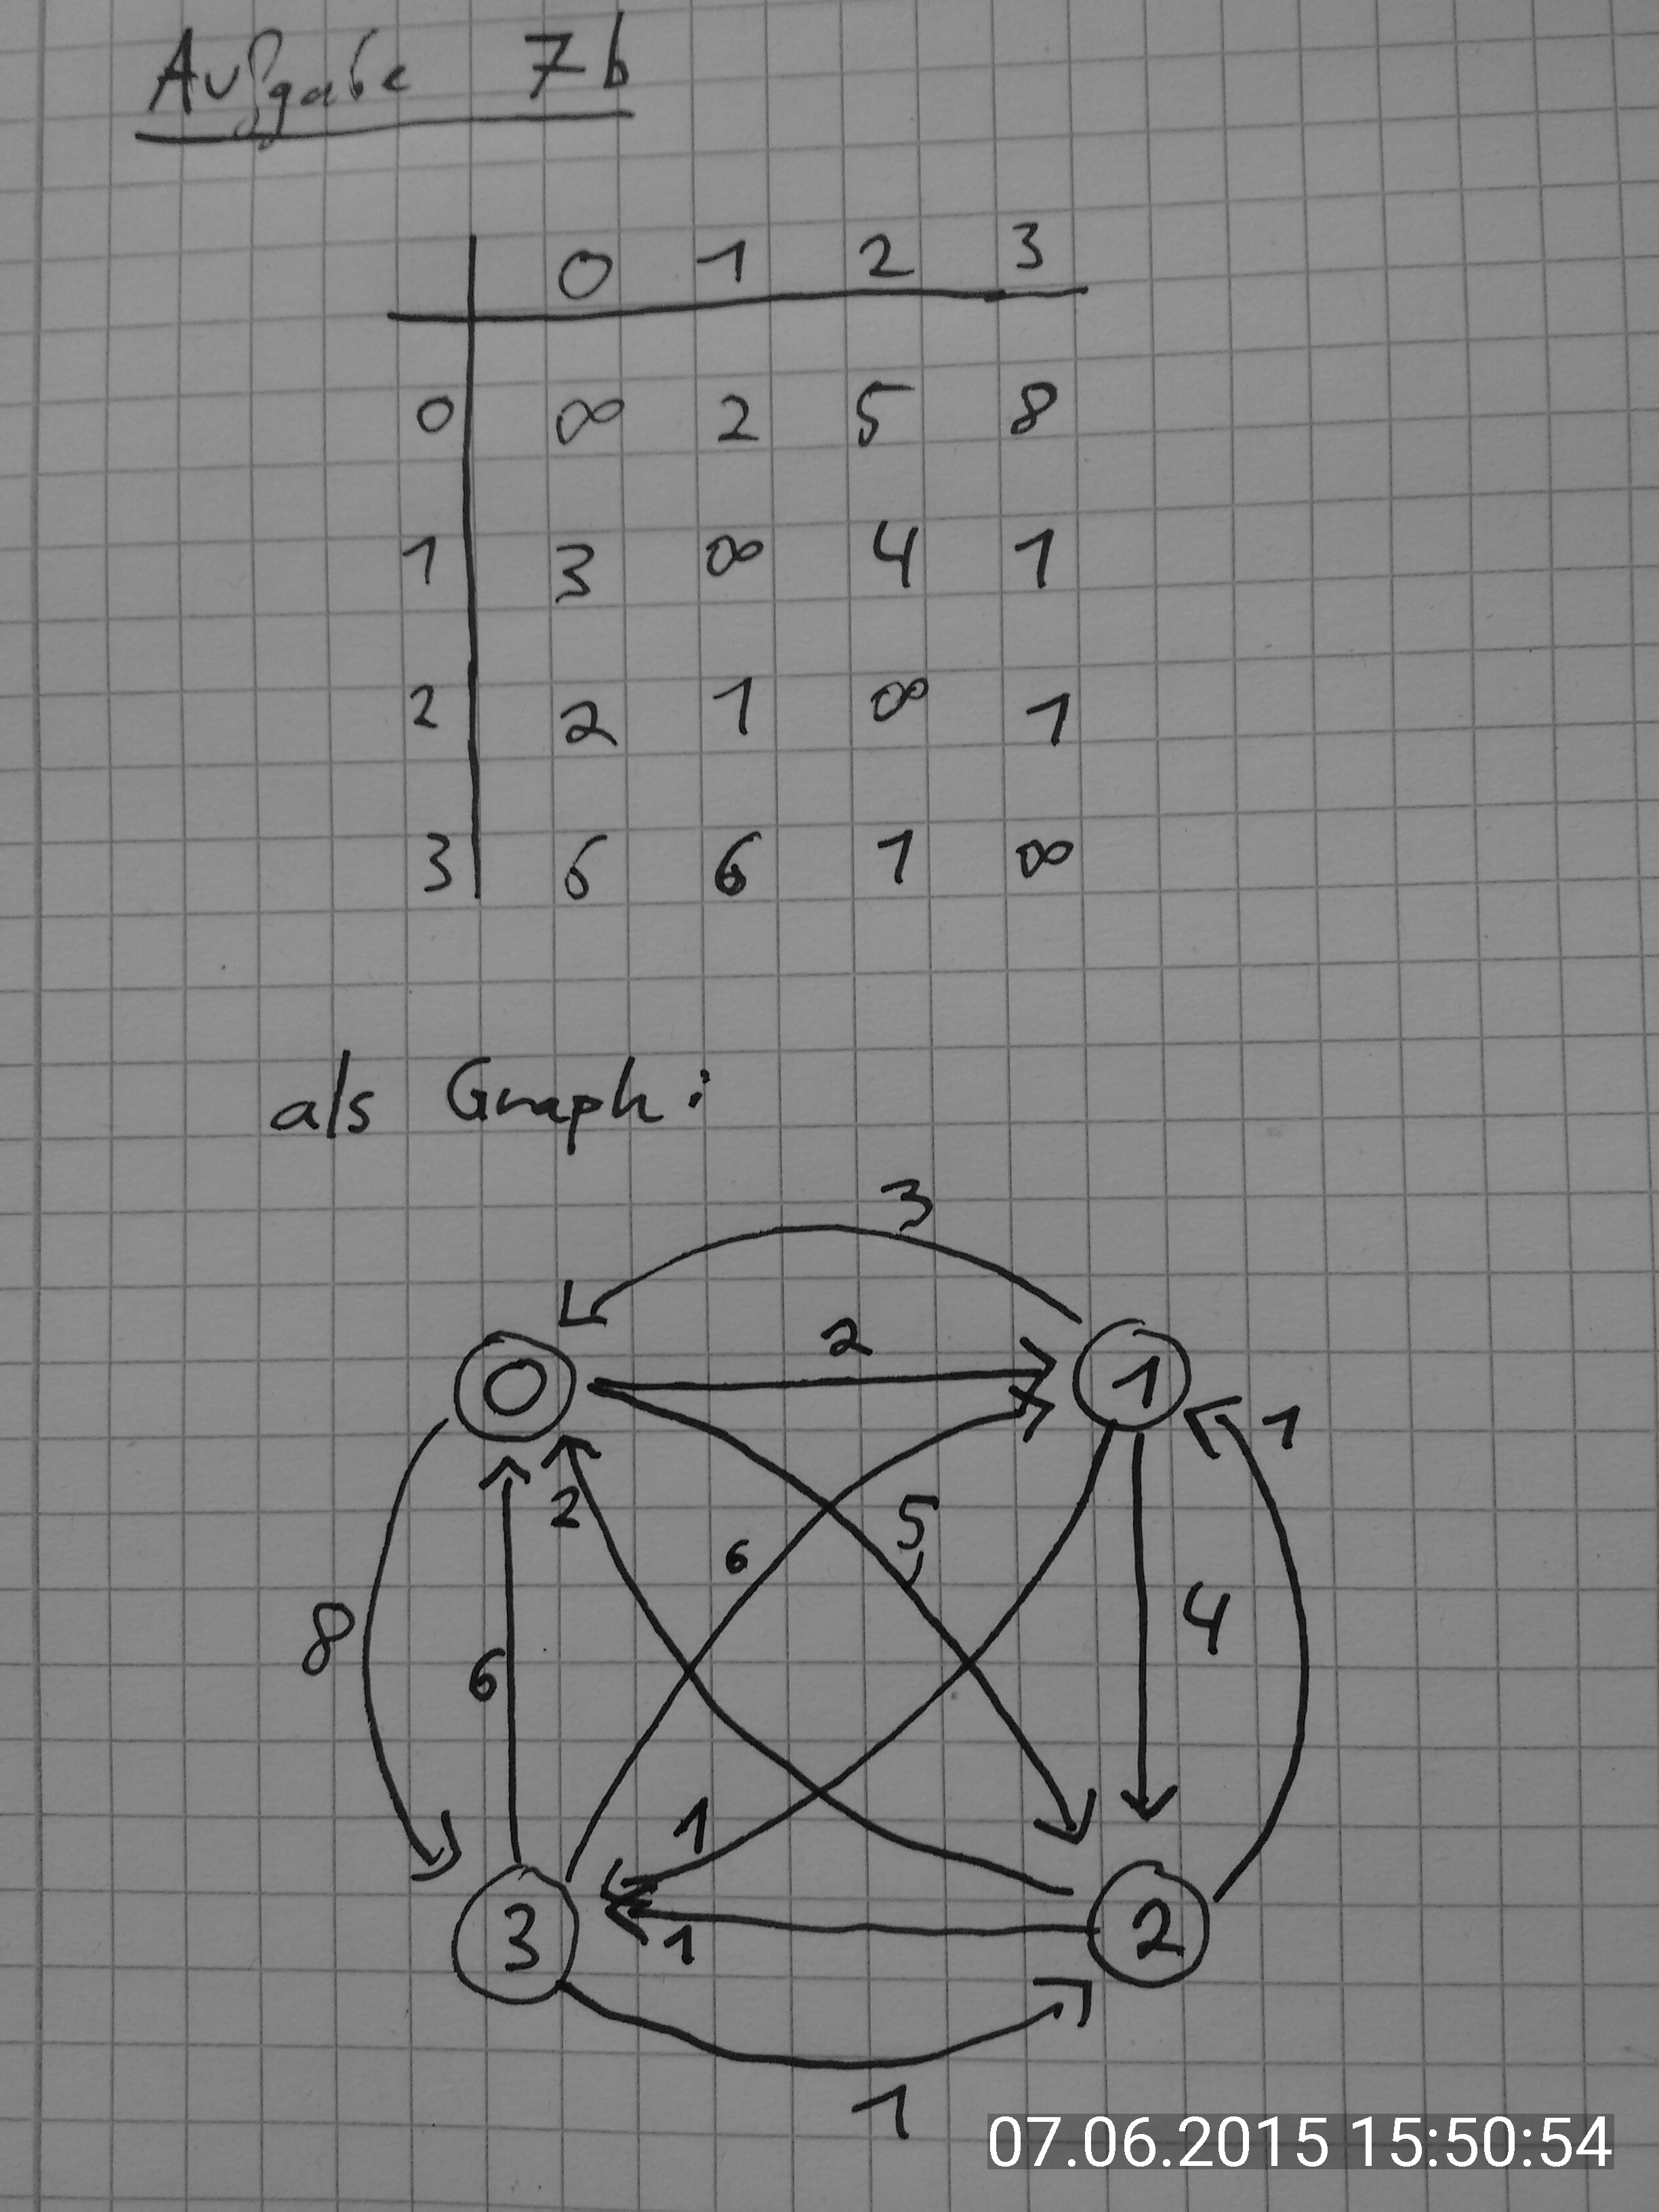
\includegraphics{01_07b1.jpg}
                }
            \end{figure}
            Die minimalen Kosten betragen nach s. 10 des Skripts:
            $$
                c_0 = 0.5 \cdot \sum_{i=0}^{n-1}
                \left( \min\limits_{j \neq i} c(j,i) +
                \min\limits_{l \neq i} c(i,l) \right)
            $$
            Das ist in unserem Fall:
            $$
                c_0 = \frac{1}{2} \cdot
                    ((2+2)+(1+1)+(1+1)+(1+1))
                    = 5
            $$
            \begin{figure}[H]
                \centering
                \def\svgwidth{\columnwidth}
                \resizebox{0.5\textwidth}{!}{
                    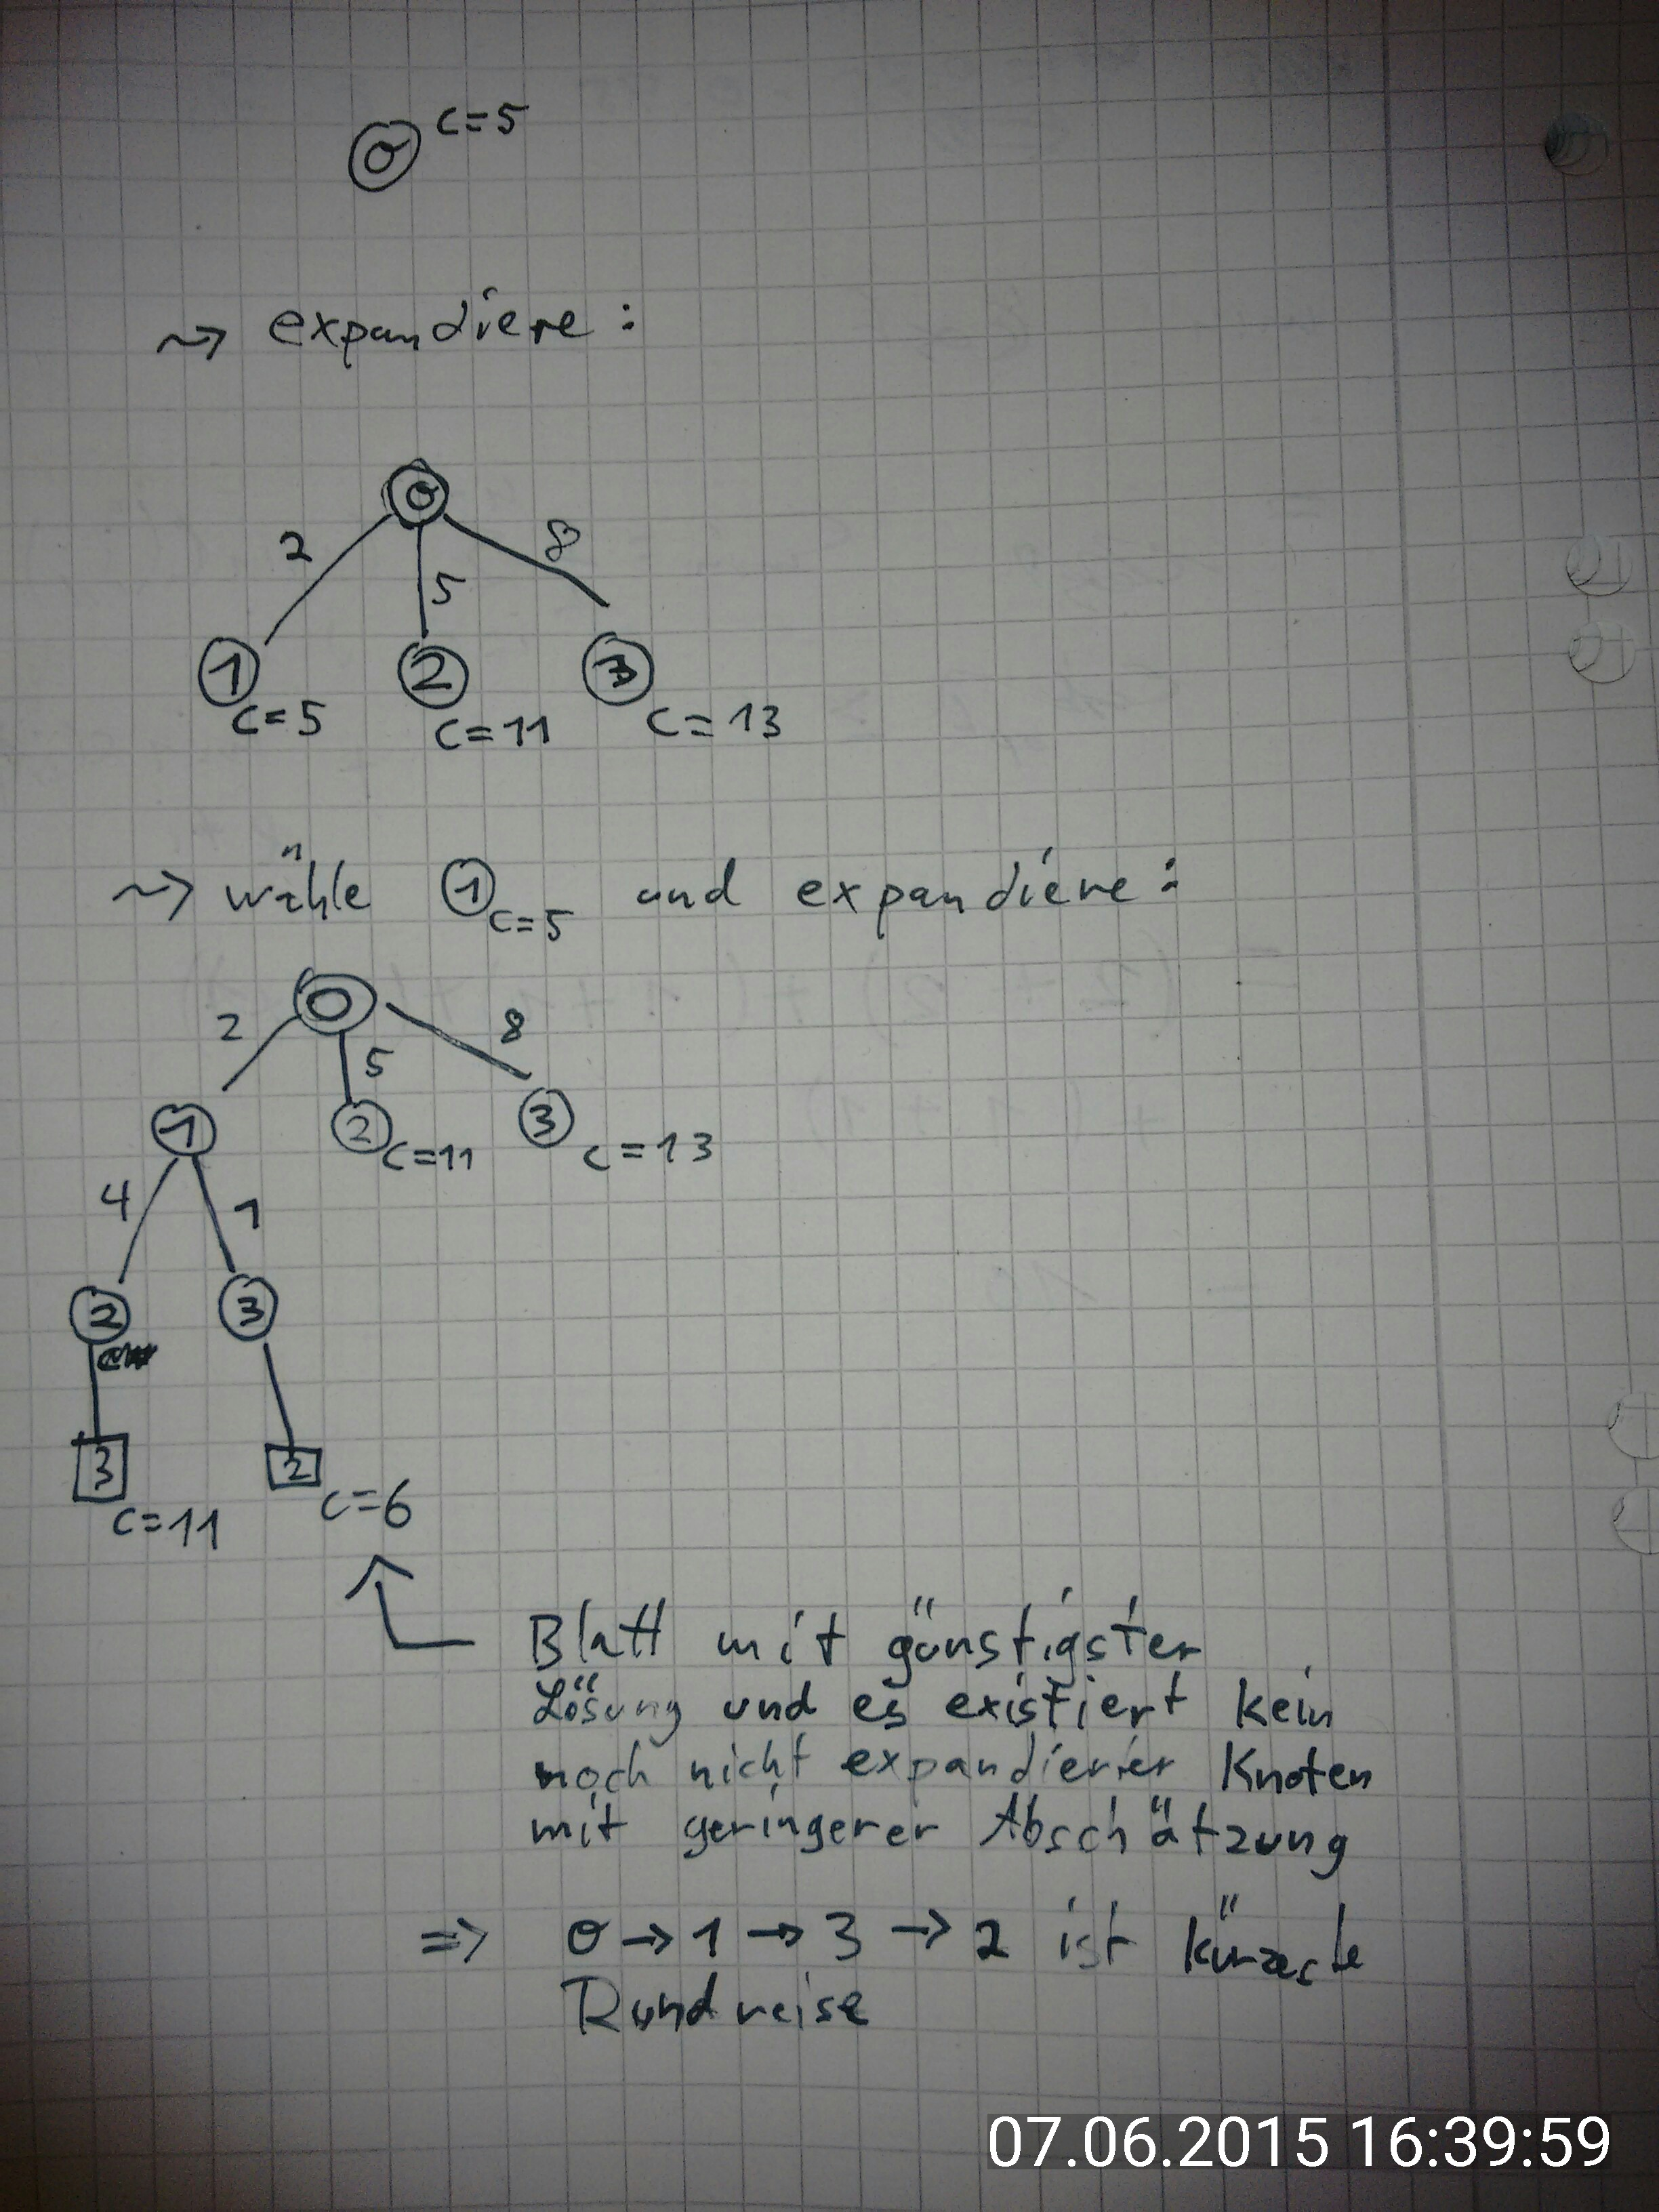
\includegraphics{01_07b2.jpg}
                }
            \end{figure}

    \end{enumerate}


\section*{Aufgabe 08}
    Seien ${p_1, p_2, \ldots, p_n}$ die Personen, die die Br\"ucke \"uberqueren
    sollen. Die Kosten f\"ur einen Lauf zur anderen Seite der Personen seien
    $c_1, c_2, \ldots, c_n$. Sei $c_{1st}$ die Kosten der schnellsten Person
    f\"ur einen Lauf und $c_{2nd}$ die Kosten der zweitschnellsten Person
    f\"ur einen Lauf. Dann k\"onnen wir die Zeit nach unten hin absch\"atzen mit:
    $$
        c_{min} = (n-1) \cdot c_{2nd} + (n-1) \cdot c_{1st}
    $$
    (Anm: $\mathbf{(n-1) \cdot c_{2nd}}$ f\"ur die ``Hinwege'',
    $\mathbf{(n-1) \cdot c_{1st}}$ f\"ur die ``R\"uckwege'') \\
    Um uns die Sache einfacher zu machen, definieren wir uns einen Knoten
    im Aufz\"ahlungsbaum als Zustand und speichern daher auch alle
    Werte, die wir zum Aufz\"ahlen des Knotens brauchen in denselben.
    Die Kosten des Knotens werden durch $c(v)$ mit $v \in V$ beschrieben
    (Keine Ahnung, wie das im Skript genau definiert ist, deshalb schreibe ich
    es hier noch mal hin; Gez. Jonas).
    Desweiteren definieren wir LS (f\"ur linke Seite) als die Start-,
    und RS als die Endseite der Br\"ucke.
    Ein Knoten hat als Attribute die Mengen L (mit den Personen auf der
    linken Seite) und R (mit den Personen auf der Rechten Seite).
    Zudem definieren wir den Startzustand so, dass die schnellste Person
    zu Beginn auf der Seite RS mit der Taschenlampe steht (das erspart
    uns eine Fallunterscheidung, die resultierenden Kosten beinhalten dann zusätzlich
    den Lauf der schnellsten Person von RS nach LS. Um das Problem in der ursprünglichen
    Aufgabenstellung zu lösen müssen diese Kosten vom Endergebnis einfach abgezogen werden)
    und die Iterationstiefe i. Ein Iterationsschritt (= einer Kante von einem
    Knoten v nach v') besteht aus zwei Schritten:
    \begin{itemize}
        \item Die Person in v.R mit minimalen Kosten l\"auft mit der Lampe nach
              v'.L (wir gehen ohne Beweis davon aus, dass diese Strategie immer
              zu keinem schlechteren Resultat als andere Aktionen f\"uhren)
        \item Zwei Personen aus v.L laufen nach v'.R
    \end{itemize}
    Daraus resultieren f\"ur v' folgende Attribute:
    \begin{itemize}
        \item v'.i = v.i + 1
        \item v'.L und v'.R ergeben sich aus der obigen Beschreibung
    \end{itemize}
    Bleiben noch die Kosten f\"ur v' zu aktualisieren. Dabei sei $c_{1st_r}$ in diesem
    Kontext die Kosten der schnellsten Person aus v'.R und $c_{1st_l}$ die Kosten
    der schnellsten Person aus v'.L . Dann gilt:

    $$
        c(v') = \textit{Kosten für den Pfad bis v} + (n-v.i-1) \cdot c_{1st_l} + (n-v.i-1) \cdot c_{1st_r}
    $$

    nun l\"asst sich das Problem mit der Kostenfunktion c(v) f\"ur jeden
    Knoten v ganz normal mit branch and bound l\"osen.




\section*{Aufgabe 09}
    \begin{enumerate}[label={\alph*)}]
        \item Handlungsreisendenproblem mit Dreiecksungleichung ($\Delta HR$): \\
            gegeben ist:
            \begin{itemize}
                \item $G = (V,E)$
                \item $V = \left\{0,1,\ldots, n-1\right\}$
                \item $c: E \rightarrow \mathbb{N}_0 $ mit:
                    \begin{itemize}
                        \item $c(i,j) = c(j,i) \forall i,j \in V$ (Symmetrie)
                        \item $c(i,j) \leq c(i,k) + c(k,j)$ (Dreiecksungleichung)
                    \end{itemize}

            \end{itemize}

            Aus Symmetrie und Dreiecksungleichung folgt: $E = V \times V
            \setminus \{ (i,i) | i \in V \} $

            gesucht ist:
            \begin{itemize}
                \item kürzeste Rundreise $\Leftrightarrow$
                    Permutation $\pi$ von $\left\{0,1,\ldots, n-1\right\}$ die
                    $$
                        \sum_{i=0}^{n-1} c(\pi(i), \pi(i+1 \mod n))
                    $$
                    minimiert.
            \end{itemize}

        \item Algorithmus ``$APPROX \Delta HR$'' aus der Vorlesung (Seite 253):
            \begin{itemize}
                \item \textbf{Eingabe:} Graph wie in \textbf{a)} beschrieben
                \item \textbf{Ausgabe:} Rundreise R mit $c(R) \leq 2 \cdot Cost_{opt}$
                \item \textbf{Algo in Textueller Beschreibung:} \\
                    \begin{itemize}
                        \item Konstruiere minimalen überspannenden Baum T(V,A)
                        \item Starte in Wurzel von T und besuche mittels Tiefensuche
                            auf T alle Knoten in V.
                        \item Schreibe die Knoten in der Reiehenfolge auf, in der
                            sie oberster Knoten im Tiefensuche-Keller sind. Dies
                            ergibt eine Knotenfolge $v_0,\ldots,v_i,\ldots,
                            v_{j-1},v_j,v_{j+1},\ldots,v_{2(n-1)-1} = v_0$.
                        \item Streiche $v_j$ genau dann aus der Knotenfolge, wenn
                        $ j < 2(n-1) + 1 $ und $ i < j $ mit $ v_i = v_j$ existiert.
                        \item gib resultierende Knotenfolge aus.
                    \end{itemize}

            \end{itemize}




    \end{enumerate}


\section*{Aufgabe 10}
    Las-Vegas und Monte-Carlo Algorithmen sind beide
    probabilistische Algorithmen. Algorithmen die Zufallszahlen
    bzw. Zufallsentscheidungen verwenden, heißen probabilistisch
    oder auch randomisiert. Las-Vegas Algorithmen liefern stets
    eine korrekte Lösung, hingenen liefern Monte-Carlo Algorithmen
    manchmal inkorrekte Lösung, deren Wahrscheinlichkeit aber sehr klein ist

\section*{Aufgabe 11}
    \begin{enumerate}[label={\alph*)}]
        \item
         Die Implementierung für randomisiertes Quicksort
         unterscheidet sich von Quicksort aus Algo 1 durch die
         Auswahl des Pivotelements. Dieses wird durch die Auswahl
         einer Zufälligen Array-Stelle, der zu betrachtenen bestimmt.
         \item
          Im worst-case ist in jedem Rekursionsschritt das Pivotelement
          das o.B.d.A. größte, s.d. ein Array in ein $(n-1)$-elementiges
          im nächsten Rekursionsschritt wird. In einem Rekursionsschritt
          müssen alle elemente verglichen werden $\Rightarrow$ $O(n)$ dadurch dass immer
          nur es ein element weniger gibt wird es $O(n)$ Rekursionsschritte
          geben.
          \\$\Rightarrow$ $O(n)\cdot O(n) = O(n^2)$
        \item
        \begin{itemize}
            \item $[123456] \looparrowright p=6$
            \item $[12345] [6] \looparrowright p=5$
            \item $[[1234] [5]] [6] \looparrowright p=4$
            \item $[[[123] [4]] [5]] [6] \looparrowright P=3$
            \item $[[[[12] [3]] [4]] [5]] [6] \looparrowright p=2$
            \item $[[[[[1] [2]] [3]] [4]] [5]] [6]$
        \end{itemize}
        \item TODO

    \end{enumerate}


\section*{Aufgabe 12}

    \begin{enumerate}[label={\alph*)}]
        \item $\zz$ RandFind korrekt: \\
        \textbf{Beweis: } durch verallgemeinerte vollständige Induktion: \\
        \begin{itemize}
            \item \textbf{IA:} n = 1 $\Rightarrow x_1$ returned $\Rightarrow $ \checkmark
            \item \textbf{IV:} $\zz$ Behauptung gilt für ein $n \in \mathbb{N}$
            \item \textbf{IS: } $n \rightarrow n + 1$ \\
                \begin{itemize}
                    \item \textbf{Fall 1:} $| S_<| = k-1$ \\
                        $\Rightarrow$ Das k. kleinste Element muss $x_i$ sein.
                    \item \textbf{Fall 2:} $|S_>| \geq k$ \\
                        $\Rightarrow $ das k. kleinste Element befindet sich in $S_<$\\
                        $\Rightarrow_{IV} $ RandFind($S_<$,k ) mit $|S_<| < n$ findet gesuchtes Element.
                    \item \textbf{Fall 3:} $|S_<| < k-1$ \\
                        $\Rightarrow$ das k. kleinste Element befindet sich in $S_>$\\
                        $\Rightarrow_{IV}$ RandFind($S_>$,k ) mit $|S_>| < n$ findet gesuchtes Element.
                \end{itemize}

        \end{itemize}
        
        \item
            In Jedem Schritt wird die noch zu betrachtenene Menge mit dem zufällig ausgewählten
            Element verglichen. oBdA Im worst-case wird zufällig immer das größte Element ausgesucht wobei
            das kleinste gesucht ist. Es wird $O(n)$ Vergleich bei$ O(n)$ Rekursionsschritten geben
            $\Rightarrow O(n)*O(n)= O(n^2)$
            
        \item TODO...
    \end{enumerate}

\section*{Aufgabe 13}
    \textbf{gegeben}: $n \in \mathbb{N}$ \\
    \textbf{Frage}: Ist n eine Primzahl? \\
    \textbf{Bemerkung}:  Offensichtlicher Primzahltest mittels Division durch alles Primzahlen n ist für große n zu ineffizient.\\
    \textbf{Ziel}: Entwicklung eines effizienten Monte-Carlo Algorithmus für den Primzahltest.\\
    \textbf{Idee}:
    \begin{itemize}
        \item 
            Entwicklung eines Kriteriums, dass für eine beliebige zusammengesetzte Zahl $n \in \mathbb{N} $ 
            und $a \in \mathbb{N}$ mit $ggT(a,n)=1$, falls es zutrifft, beweist, dass $n$ zusammengesetzt ist.
        \item
            Beweis, dass im Fall n zusammengesetzt, höchstens ein Viertel der 
            natürlichen Zahlen $a<n$ mit$ ggT(a,n)=1$ das Kriterium \textbf{nicht} erfüllt
        \item
            falls n eine Primzahl ist, dann ist das Kriterium nie erfüllt.
            
    \end{itemize}
    \textbf{Textueller Algo:}\\
        \begin{algorithm}[H]
            wähle $a<n$\;
            \For{t \KwTo $k \in \mathbb{N}$} {
                \If{$ggT(a,n) \neq 1 $}{
                    \textit{\# $n$ ist zusammengesetzt}\\
                    return false\;
                }
             }
           \textit{ \# wir haben für eine hinreichend große Anzahl (=k) das}\\
           \textit{ \# Kriterium getestet}\\
            return true\;
                
        \end{algorithm}

\end{document}
